\chapter{Standard Machine Learning Language} \label{Chapter:SML}

\section{Introduction}
\label{Introduction}
\blfootnote{
This chapter contains material from the following working paper: 
\nobibliography{thesisbib}
\begin{itemize}
\item\bibentry{SML}
\end{itemize}
}

Machine Learning has simplified the process of solving problems in a variety of fields (see \cite{ML-UseCase1} or \cite{Monahan} for examples).  However, \cite{pedros:fewUsefulThings} noted several nuisances to consider when developing machine learning pipelines.  If one does not consider these nuisances into consideration, one may not receive satisfactory results.  To combat these issues, we introduce Standard Machine Learning Language (SML), targeted at domain experts that want to utilize machine learning to solve research questions.

The overall objective of SML is to provide a level of abstraction which simplifies the development process of machine learning pipelines.  Consequently, this will enable students, researchers, and industry professionals without a background in developing machine learning pipelines to solve problems in different domains with machine learning (see Listing \ref{lst:sml-ex-1} for an example).  In the subsequent sections, related works are discussed,  followed by defining the grammar used to create SML queries. The architecture of SML is described. Lastly, SML is applied to use-cases to demonstrate how it reduces the complexity of solving problems that utilize machine learning.

\section{Prior Works}
\label{SML:PriorWorks}

There are prior related works that attempt to provide a level of abstraction for developing machine learning models.  \cite{RizzoloRo10} created a tool called LBJava based on a programming paradigm called Learning Based Programming (see \cite{Roth05}). Learning Based Programming is an extension of conventional programming that creates functions using data-driven approaches.  LBJava utilizes machine learning to create these functions and abstract the details from the user.  What differentiates SML from LBJava is that it offers a higher level of abstraction by providing a query-like language, allowing people who aren't experienced programmers to use SML.  

TPOT (see \cite{TPOT}) is a tool implemented in Python that creates and optimizes machine learning pipelines using genetic programming.  Given cleaned data,  TPOT  preprocessing the data,  performs feature selection,  and the construction of machine learning models.  Given the task (classification,  regression,  or clustering) TPOT uses genetic programming to tune model parameters and select features to determine the most optimal model to use.  Similar to TPOT \cite{kotthoff_auto_2019} developed Auto-WEKA, which automates the selection of learning algorithms and tuning hyper-parameters for implemented models in WEKA see (\cite{frank2005weka}).   

Subsequently \cite{komer_hyperopt_2019} created Hyperopt-Sklearn that provides automated algorithm selection from models in the Scikit-learn machine learning library \footnote{See \cite{scikit-learn} for an introduction to Scikit-learn.} similar to Auto-Weka.  \cite{feurer_auto_2018} introduced improvements upon Hyperopt-Sklearn by taking into account past performance on similar datasets and constructing ensembles from optimized models.  What differentiates SML from these prior works is that it provides an agnostic language to reduce the amount of programming required to write and offers a visualization framework to assess the models' performance visually.

\section{Grammar}
\label{grammar}

The SML language is a domain-specific language with grammar implemented in Bakus-Naur form (BNF) (see \cite{Backus59}).  Each expression has a rule and can be expanded into additional terms.  Listing \ref{lst:sml-ex-1} is an example of how one would perform classification on a dataset using SML. The query in listing \ref{lst:sml-ex-1} reads from a dataset, performs an 80/20 split of training and testing data, respectively, and performs classification on the 5th column of the hypothetical dataset using columns 1,2,3, and 4 as predictors. In the subsequent subsections, SML's grammar in BNF form is defined in addition to the keywords.

\subsection{Grammar Structure}
This subsection is dedicated to defining the grammar of SML in terms of BNF.  A \(Query\) can be defined by a delimited list of actions where the delimiter is an \(AND\) statement; with BNF syntax this is defined as:

\begin{equation} \label{BNF:Query}
<Query> ::= <Action> | <Action> AND <Query>
\end{equation}

An \(Action\) in (\ref{BNF:Query}) follows one of the following structures defined in (\ref{BNF:Action}) where a \(Keyword\) is required followed by an \(Argument\) and/or \(OptionList\).

\begin{equation} \label{BNF:Action}
\begin{split}
<Action> ::= <Keyword> <Argument> \\
| <Keyword> <Argument> (<Option List>) \\
| <Keyword> (<Option List>)
\end{split}
\end{equation}

A \(Keyword\) is a predefined term associating an \(Action\) with a particular string. An \(Argument\) generally is a single string surrounded by quotes that specifies a path to a file. Lastly,  an \(Argument\) can have a multitude of options (\ref{BNF:Option}) where an \(Option\) consist of an \(OptionName\) with either an \(OptionValue\) or \(OptionValueList\). An \(OptionName\) and \(OptionValue\) consist of a single string. An \(OptionList\) (\ref{BNF:OptionList}) consist of a comma delimited list of options and an \(OptionValueList\) (\ref{BNF:OptionValueList}) consist of a comma delimited list of \(OptionValues\).

\begin{equation} \label{BNF:Option}
\begin{split}
<Option> ::= <Option Name> = <Option Value> \\
		| <Option Name> = [<Option Value List>]
\end{split}
\end{equation}

\begin{equation} \label{BNF:OptionList}
\begin{split}
	<Option List> ::= <Option> | <Option>,  <Option List>
\end{split}
\end{equation}

\begin{equation} \label{BNF:OptionValueList}
\begin{split}
<Option Value List> ::= <Option Value> \\
| <Option Value> ,  <Option Value List>
\end{split}
\end{equation}

To put the grammar into perspective the example \(Query\) in Listing \ref{lst:sml-ex-1} has been transcribed into BNF format and can be found in Listing \ref{lst:SML:BNFComp}. In  Listing \ref{lst:SML:BNFComp}  the first \(Keyword\) is \(READ\) followed by an \(Arugment\) that specifies the path to the dataset. Next, an \(OptionValueList\) contains information about the delimiter of the dataset and the header. We include the \(AND\) delimiter to specify an additional \(Keyword\) \(SPLIT\) with an \(OptionValueList\) that tells us the size of the training and testing partitions for the dataset specified with the \(READ\) \(Keyword\). Lastly,  we use the \(AND\) delimiter to specify another \(Keyword\) \(CLASSIFY\) which performs classification using the training and testing data from the result of the  \(SPLIT\) \(Keyword\) followed by an \(OptionValueList\) which provides information to SML about the features to use (columns 1-4), the label we want to predict (column 5), and the algorithm to use for classification. The next subsection describes the functionality for all \(Keyword\)s of SML.

\subsection{Keywords}
Currently, there are eight \(Keyword\)s in SML \footnote{Detailed documentation providing examples and describing all of the keywords of SML are publicly available on GitHub: https://github.com/lcdm-uiuc/sml/tree/master/dataflows \label{SML:Dataflow}}. These \(Keyword\)s can be chained together to perform a variety of actions. In the subsequent subsections, we describe the functionality of each \(Keyword\).

\subsubsection{Reading Datasets}
When reading data from SML one must use the \(READ\) \(Keyword\) followed by an \(Argument\) containing a path to the dataset. \(READ\) also accepts a variety of \(Option\)s. The first \(Query\) in listing \ref{lst:SML:READ} consist of only a \(Keyword\) and \(Argument\). This \(Query\) reads in data from "/path/to/dataset". The second \(Query\) includes an \(OptionValueList\) in addition to reading data from the specified path; the \(OptionValueList\) specifies that the dataset is delimited with semicolons and does not include a header row. 


\subsubsection{Cleaning Data}
When NaNs, NAs, and other missing values are present in the dataset, we clean these values in SML by using the \(REPLACE\) \(Keyword\).  Listing \ref{lst:SML:REPLACE}  shows an example of the \(REPLACE\) \(Keyword\) being used. In this \(Query\) we use the \(REPLACE\) \(Keyword\) in conjunction with the \(READ\) \(Keyword\).  SML reads from a comma-delimited dataset with no header from the path "/path/to/dataset". Then we replace any instance of "NaN" with the mode of that column in the dataset.


\subsubsection{Partitioning Datasets}
It is often useful to split a dataset into training and testing datasets for most tasks involving machine learning.  Splitting a dataset can be achieved in SML by using the \(SPLIT\) \(Keyword\).  Listing \ref{lst:SML:SPLIT} shows an example of a SML \(Query\) performing an 80/20 split for training and testing data respectively by utilizing the \(SPLIT\) \(Keyword\) after reading in data.

\subsubsection{Creating Models}

In SML,  one can create a model to either perform classification, regression, or clustering. To use a classification model in SML one would use the \(CLASSIFY\) \(Keyword\). SML has the following classification models implemented: Support Vector Machines, Naive Bayes, Random Forest, Logistic Regression, and K-Nearest Neighbors.  Listing \ref{lst:SML:CLASSIFY} demonstrates how to use the \(CLASSIFY\) \(Keyword\) in a \(Query\).  Clustering models can be utilized by using the \(CLUSTER\) \(Keyword\).  SML currently has K-Means clustering implemented.  Listing \ref{lst:SML:CLUSTER} demonstrates how to use the \(CLUSTER\) \(Keyword\) in a \(Query\).  Regression models use the \(REGRESS\) \(Keyword\).  SML currently has the following regression algorithms: Simple Linear Regression, Ridge Regression, Lasso Regression, and Elastic Net Regression. Listing \ref{lst:SML:REGRESS} demonstrates how to use the \(REGRESS\) \(Keyword\) in a \(Query\).


\subsubsection{Saving/Loading Models}
It is possible to save models and reuse them later. To save a model in SML one would use the \(SAVE\) \(Keyword\) in a \(Query\). To load an existing model from SML one would use the \(LOAD\) \(Keyword\) in a \(Query\).  Listing \ref{lst:SML:SAVE_LOAD} shows the syntax required to save and load a model using SML.  With any of the existing queries using \(REGRESS\),  \(CLUSTER\),  or \(CLASSIFY\) \(Keyword\)s attaching \(SAVE\) to the \(Query\) will save the model. 

\subsubsection{Visualizing Datasets and Metrics of Algorithms}
When using SML it is possible to visualize datasets or performance of models (such as learning curves or ROC curves).  To do this, the \(PLOT\) \(Keyword\) must be specified in a \(Query\).  Listing \ref{lst:SML:PLOT} shows an example of how to use the \(PLOT\) \(Keyword\) in a \(Query\).  We apply the same operations to perform clustering in Listing \ref{lst:SML:CLUSTER} however, we utilize the \(PLOT\) \(Keyword\).

\section{SML's Architecture}
\label{sml-architecture}

With SML's grammar defined, we have presented enough information to explain SML's architecture.  When SML receives a \(Query\) in the form of a string, it is passed to the parser. The grammar parses through the string to determine the actions to perform.  The actions are stored in a dictionary and given to one of the following SML phases: Model Phase, Apply Phase, or Metrics Phase. Figure \ref{fig:SML:Architecture} shows a block diagram of this process.

The model phase is for constructing a model. The \(Keyword\)s that generally invoke the model phase are: \(READ\), \(REPLACE\), \(CLASSIFY\), \(REGRESS\), \(CLUSTER\), and \(SAVE\). The apply phase is for applying a preexisting model to new data. The \(Keyword\) that invokes the apply phase is \(LOAD\). It's often useful to visualize the data that one works with and beneficial to see a machine learning model's performance metrics. By default, if one specify the \(PLOT\) \(Keyword\) in a \(Query\), SML will execute the metrics phase.

The last significant component of SML's architecture is the connector. The connector connects drivers from different libraries and languages to achieve an action a user wants during a particular phase (see Figure \ref{fig:SML:Connector}). If one considers applying linear regression on a dataset, SML calls the connector to retrieve the linear regression library during the model phase. In this case, SML uses sci-kit learn's implementation. However, if we wanted to use an algorithm not available in sci-kit learn, such as a Hidden Markov Model (HMM), SML will use the connector to call another library that supports HMM.

\section{Interface}
\label{interface}

There are multiple interfaces available for working with SML. We have developed an alpha version of a web tool that allows users to write queries and get results back from SML through a web interface (see Figure \ref{fig:SML:website}). There is also a REPL environment available that allows the user to write queries and display results from the appropriate phases of SML interactively.  Lastly,  users can import SML into an existing pipeline to simplify the development process of applying machine learning to problems.

\section{Use Cases}
\label{use-cases}

We tested SML's framework against ten popular machine learning problems with publicly available data sets. We applied SML to the following datasets: Iris Dataset \footnote{https://archive.ics.uci.edu/ml/datasets/Iris}, Auto-MPG Dataset \footnote{https://archive.ics.uci.edu/ml/datasets/Auto+MPG}, Seeds Dataset \footnote{https://archive.ics.uci.edu/ml/datasets/seeds},  Computer Hardware Dataset \footnote{https://archive.ics.uci.edu/ml/datasets/Computer+Hardware},  Boston Housing Dataset \footnote{https://archive.ics.uci.edu/ml/datasets/Housing}, Wine Recognition Dataset \footnote{https://archive.ics.uci.edu/ml/datasets/Wine}, US Census Dataset \footnote{https://archive.ics.uci.edu/ml/datasets/US+Census+Data+(1990)}, Chronic Kidney Disease \footnote{https://archive.ics.uci.edu/ml/datasets/Chronic\_Kidney\_Disease}, Spam Detection \footnote{https://archive.ics.uci.edu/ml/datasets/Spambase} which were taken from UCI's Machine Learning Repository (see \cite{Lichman:2013}).  We also applied SML to the Titanic Dataset \footnote{https://www.kaggle.com/c/titanic}.  

As mentioned in footnote \ref{SML:Dataflow} there are detailed examples and explanations for all 10 data sets.  In this chapter, we discuss the process of applying SML to the Iris Dataset and the Auto-MPG dataset.   We compare the process for using machine learning to solve the problems presented by the datasets with SML against traditionally writing code.  We forgo comparing SML to prior works in section \ref{SML:PriorWorks}.  We used the same libraries and programming language in SML to solve these use cases for both of these datasets. 

\subsubsection{Iris Dataset}
Listing \ref{lst:SML:IrisQuery} shows all of the code required to perform classification on the Iris dataset using SML in Python.  We read in data in listing \ref{lst:SML:IrisQuery} from a specified path named "iris.csv" from a subdirectory called "data" and perform an 80/20 split, uses the first four columns to predict the fifth column, uses support vector machines as the algorithm to perform classification and finally plot distributions of features from the dataset and metrics of the classification model's performance.  Appendix \ref{Appendix:Iris} illustrates what is required to perform the same operations using Python and sci-kit learn.  The \(Query\) in listing \ref{lst:SML:IrisQuery} and the code in Appendix \ref{Appendix:Iris} use the same 3rd party libraries implicitly or explicitly.  It is also worth noting that the code in Appendix \ref{Appendix:Iris} is publicly available and well documented \footnote{For detailed documentation describing this code visit: https://github.com/lcdm-uiuc/sml/blob/master/dataflows/plot/iris\_svm-READ-SPLIT-CLASSIFY-PLOT.ipynb \label{lab:iris:git}} and it is out of the scope of this paper.  Instead the complexities required to produce such results with and without SML are outlined.  The result for both snippets of code are the same and is in Figure \ref{fig:IrisResults}.

\subsubsection{Auto-Mpg Dataset}
Listing  \ref{lst:SML:AutoMPGQuery} shows the SML \(Query\) required to perform regression on the Auto-MPG dataset in Python.  In listing \ref{lst:SML:AutoMPGQuery} we read data from a specified path, fixed-width spaces separate the dataset, and we choose not to provide a header for the dataset.  Next, we perform an 80/20 split, replace all occurrences of "?" with the column's mode. We then perform linear regression using columns 2-8 to predict the 1st label. Lastly, we visualize distributions of features from the dataset and metrics of our algorithm.  Appendix \ref{Appendix:Auto}.  demonstrates what's required to perform the same operations using sci-kit learn \footnote{For a detailed documentation describing this code visit: https://github.com/lcdm-uiuc/sml/blob/master/dataflows/plot/autompg\_linear\_regression-READ-SPLIT-REGRESS-PLOT.ipynb \label{lab:SML:AUTO}}. The outcome of both processes are the same and can be seen in Figure \ref{fig:AutoMPG:Results}.

\subsection{Discussion}
For the Iris and Auto-MPG use cases, the same libraries and programming language were used to perform regression and classification.  The amount of work required to perform a task and produce the following results in Figure \ref{fig:AutoMPG:Results} and Figure \ref{fig:IrisResults} significantly decreases when SML is utilized.  Constructing each SML query used less than 10 lines of code; however, implementing the same procedures without SML using the same programming language and libraries needed 70+ lines of code.  This provides evidence that SML simplifies the development process of solving problems with machine learning.  

\section{Future Work}
While we have formally introduced an agnostic framework, much work remains to improve SML.  In the future, we plan to extend the connector to support more machine learning libraries and additional languages.  We can extend SML's web application to include additional functionality to improve the ease of use.  Feature selection, model selection, and parameter optimization are additional areas to add to SML.  In addition to improving SML it can also be tested by researchers in a comparative analysis against the works outlined in section \ref{SML:PriorWorks} to determine how beneficial SML is against alternative frameworks.

\section{Conclusion}
\label{conclusion}
To summarize, we introduced an agnostic framework that integrates a query-like language to simplify the development of machine learning pipelines.  We provided a high-level overview of its architecture and grammar. We then applied SML to machine learning problems and demonstrated how the code one has to write significantly decreases when SML is used.  The source code and detailed documentation for SML is open-sourced and publicly available on github \footnote{https://github.com/lcdm-uiuc/sml \label{SML:Github}}. 


SML provides a realm of possibility to rapidly develop machine learning pipelines with an agnostic language to solve problems. This attractive aspect can boost the productivity of researchers who utilize machine learning.  Abstracting machine learning complexities with a tool like SML can foster new research and solve problems in different disciplines faster.

\clearpage

\section{Figures and Listings}

\rotatebox{90}{\begin{minipage}{0.95\textheight}
   \centerline{ 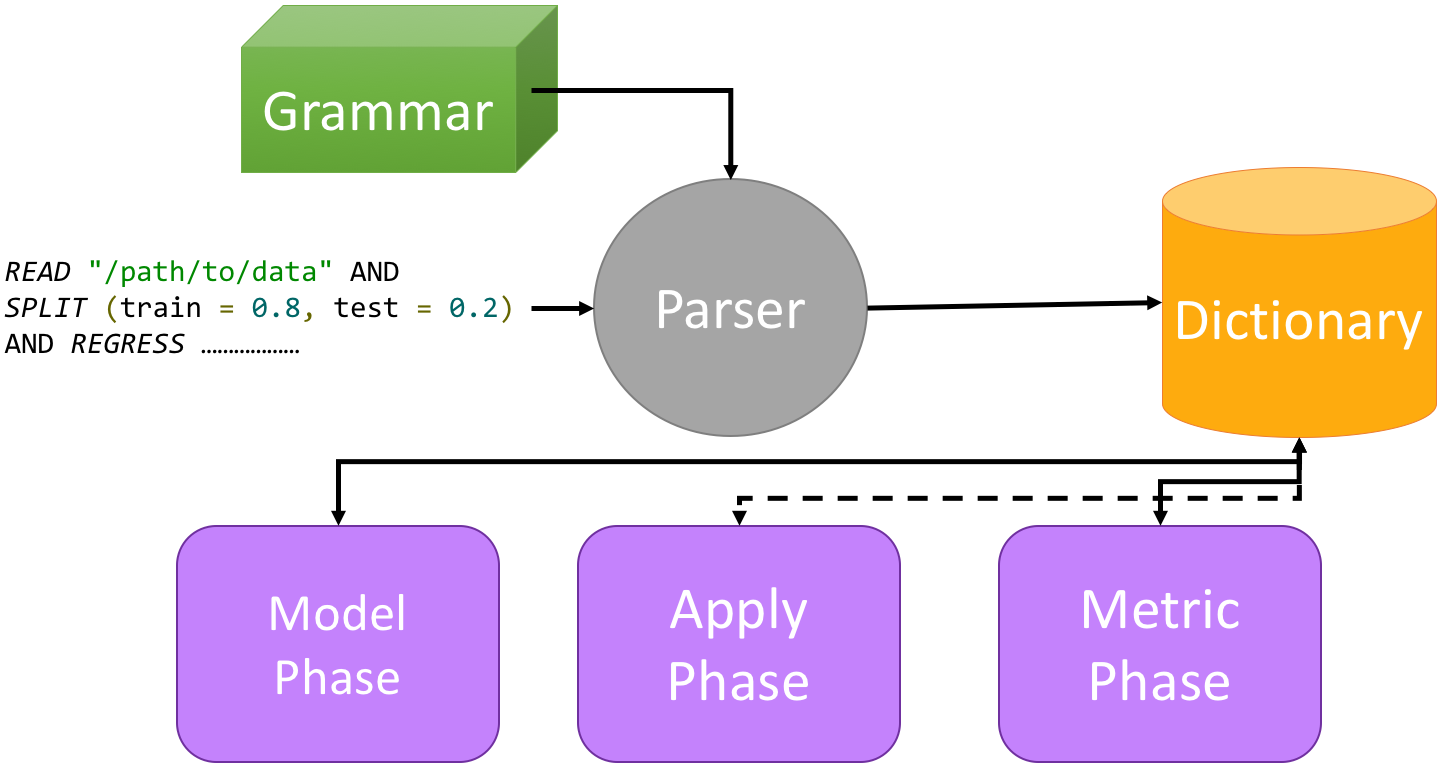
\includegraphics[width=\textwidth]{figures/SML/architecture.png}}
    \captionof{figure}{This figure shows a Block Diagram of SML's Connector.}
    \label{fig:SML:Architecture}
\end{minipage}}

%\begin{sidewaysfigure}[!h]
%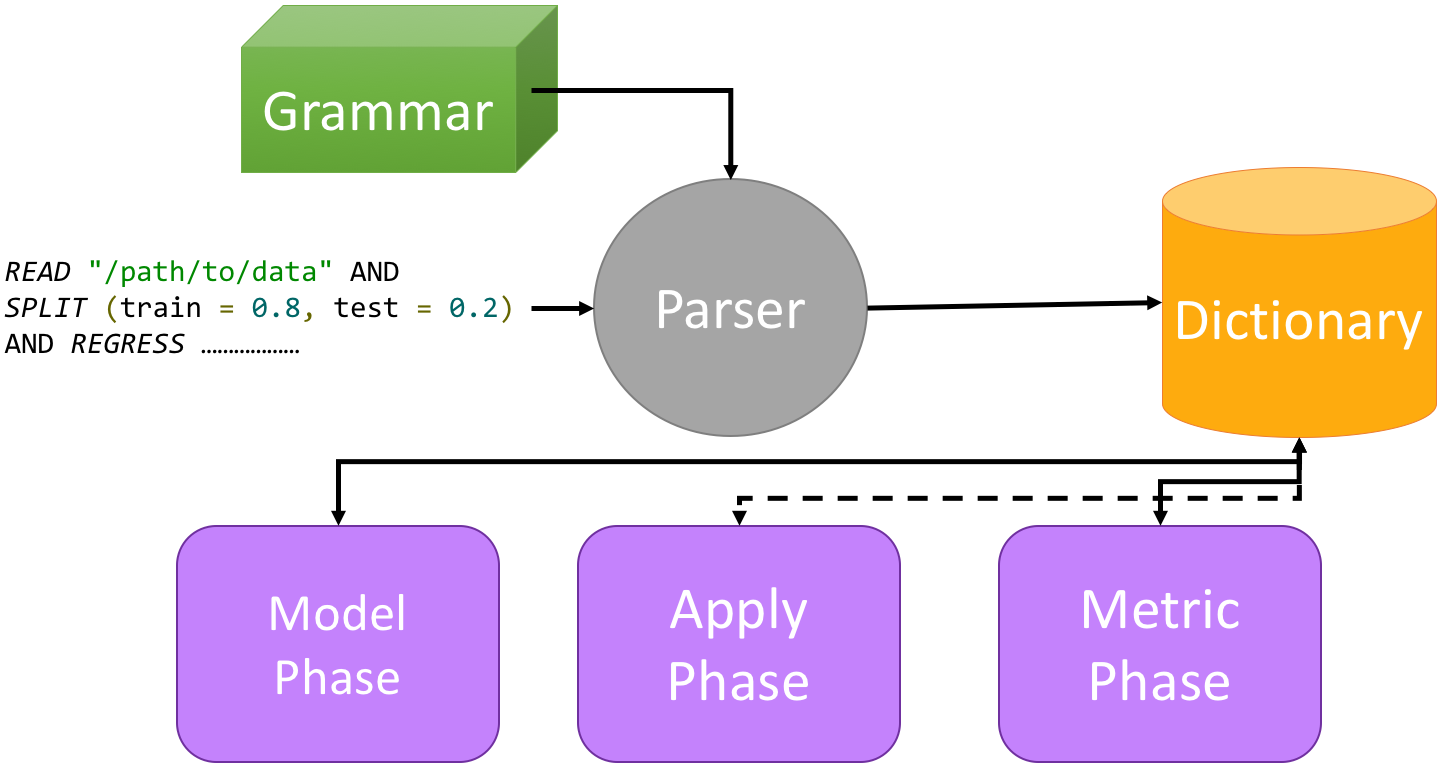
\includegraphics[width=.9\textwidth]{figures/SML/architecture.png}
%\centering
%\caption{Block Diagram of SML's Architecture\\}
%\label{fig:SML:Architecture}
%\end{sidewaysfigure}

\begin{sidewaysfigure}![h]
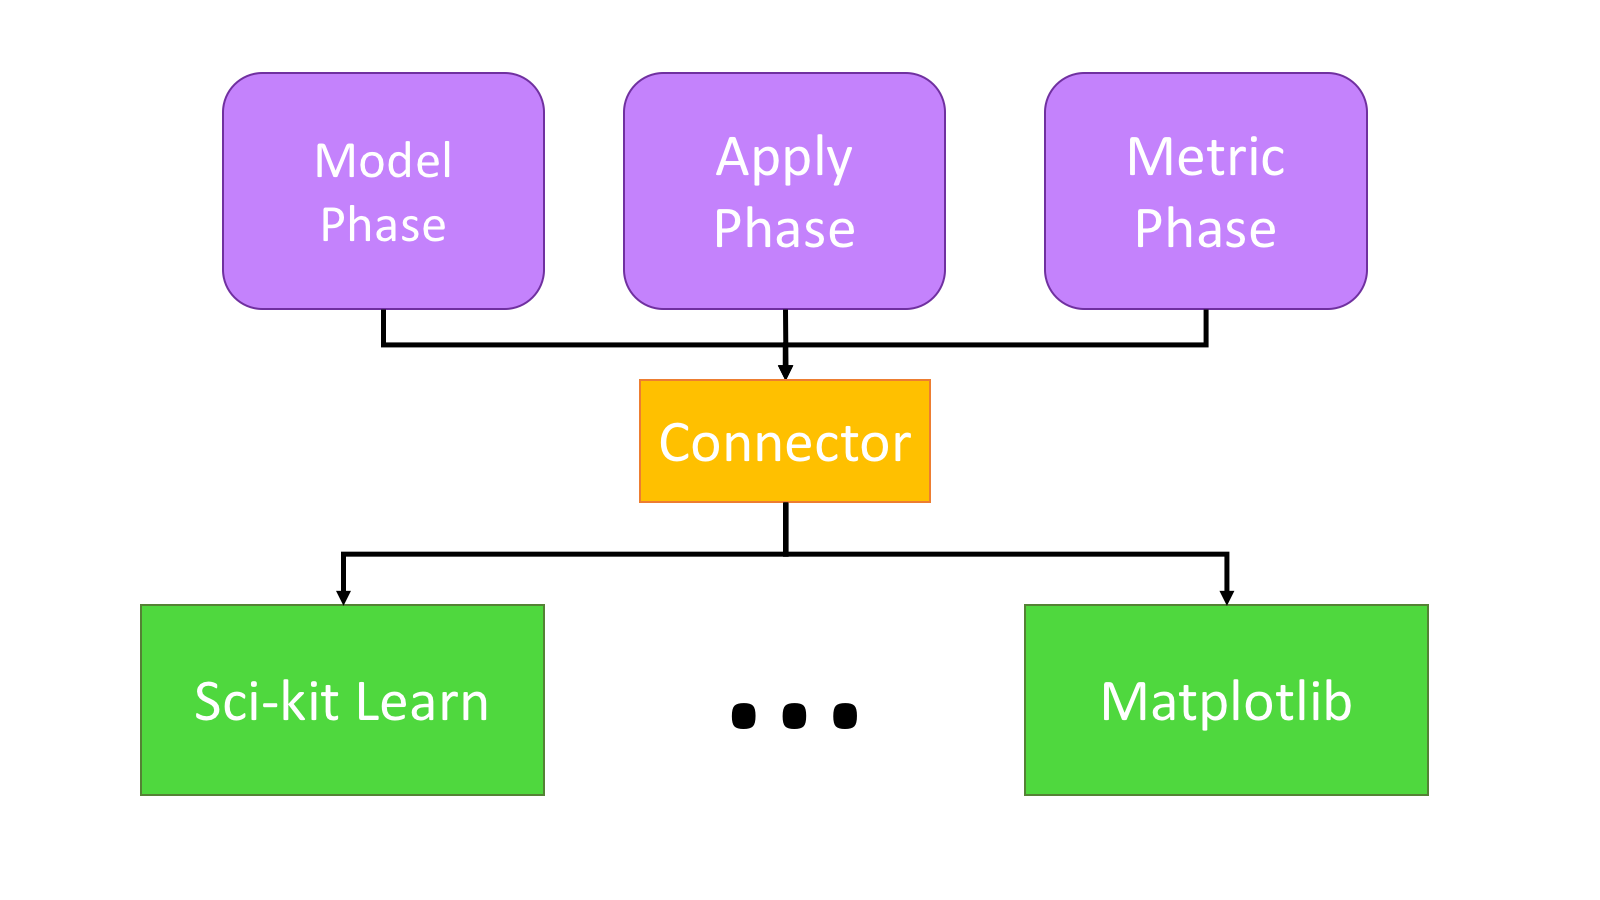
\includegraphics[width=1\textwidth]{figures/SML/connector.png}
\centering
\caption{This figure shows a Block Diagram of SML's Connector.}
\label{fig:SML:Connector}
\end{sidewaysfigure}

\begin{sidewaysfigure}[!h]
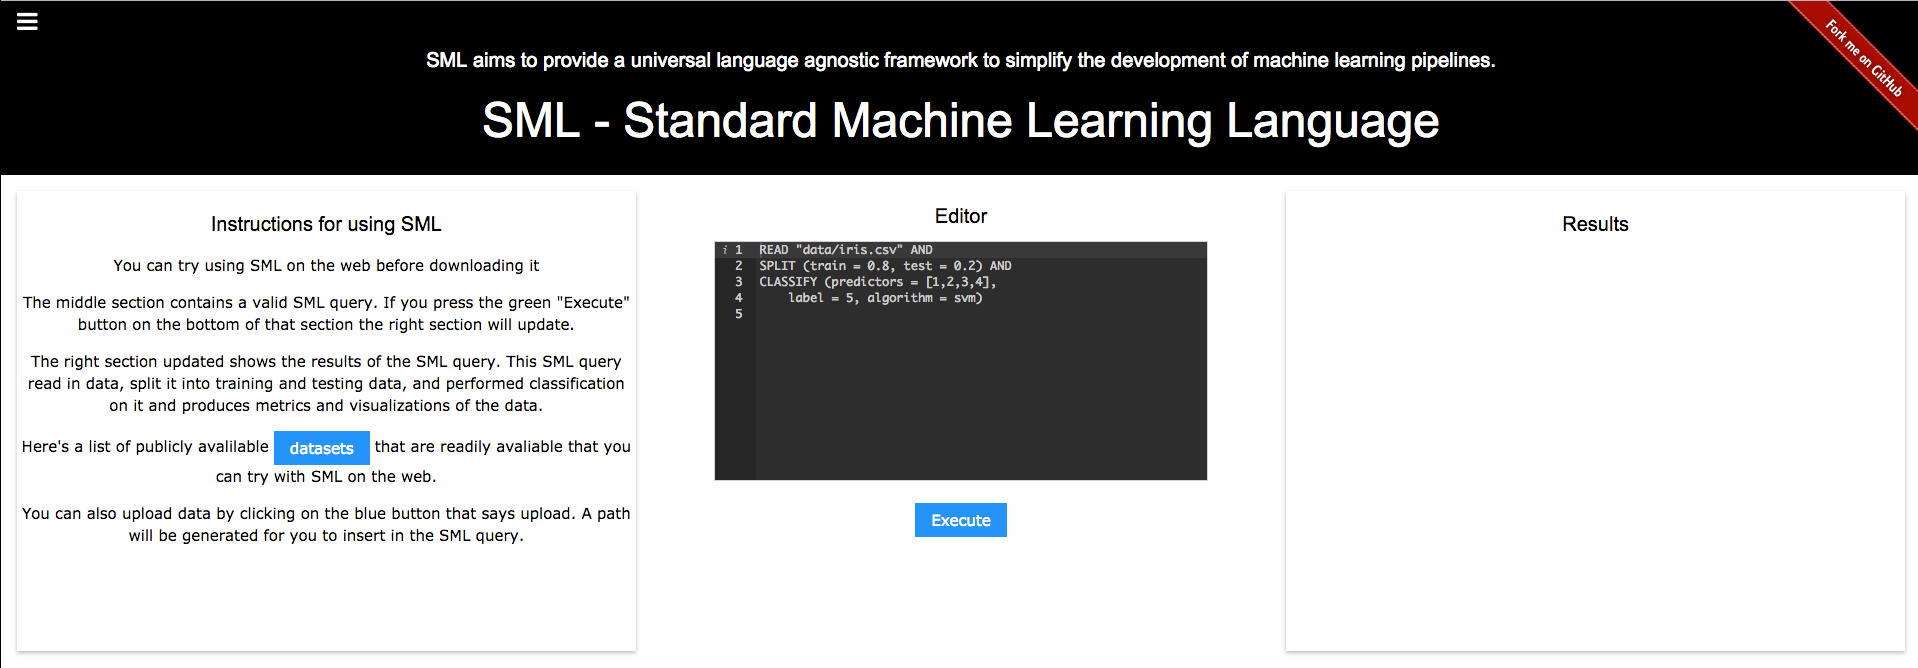
\includegraphics[width=1\textwidth]{figures/SML/sml-web-site.png}
\centering
\caption{This figure shows the interface of SML's webapp. Currently, users can read instructions, and examples of how to use SML are on the left pane. In the middle pane, users can type an SML \(Query\) and then hit the execute button. The results after executing a SML \(Query\) through SML are in the right pane.}
\label{fig:SML:website}
\end{sidewaysfigure}


\begin{sidewaysfigure}[!h]
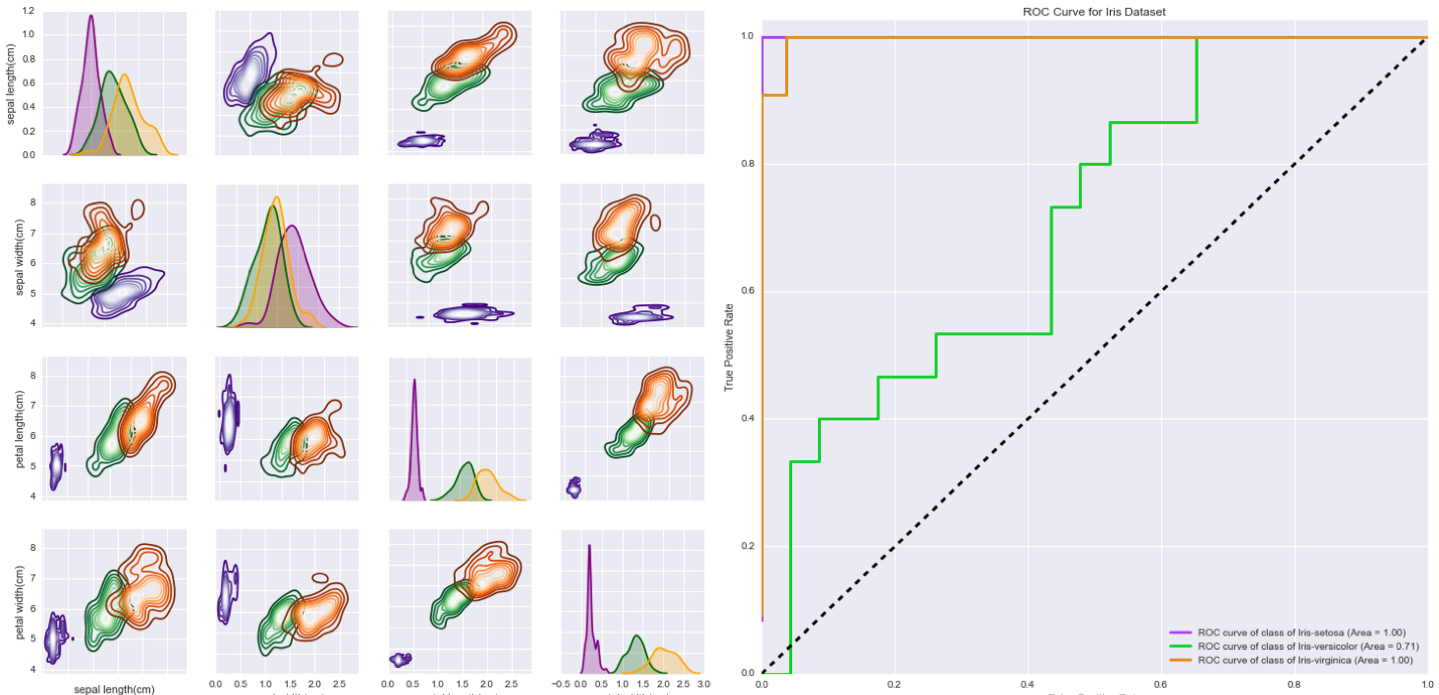
\includegraphics[width=1\textwidth]{figures/SML/iris_results.png}
\centering
\caption{The SML \(Query\) in figure \ref{fig:SML:IrisQuery} and the code in figure \ref{fig:Manual:IrisCode} produce these results. The subgraph on the left is a lattice plot showing the density estimates of each feature used. The graph on the right shows the ROC curves for each class of the iris dataset.}
\label{fig:IrisResults}
\end{sidewaysfigure}

\begin{sidewaysfigure}[!h]
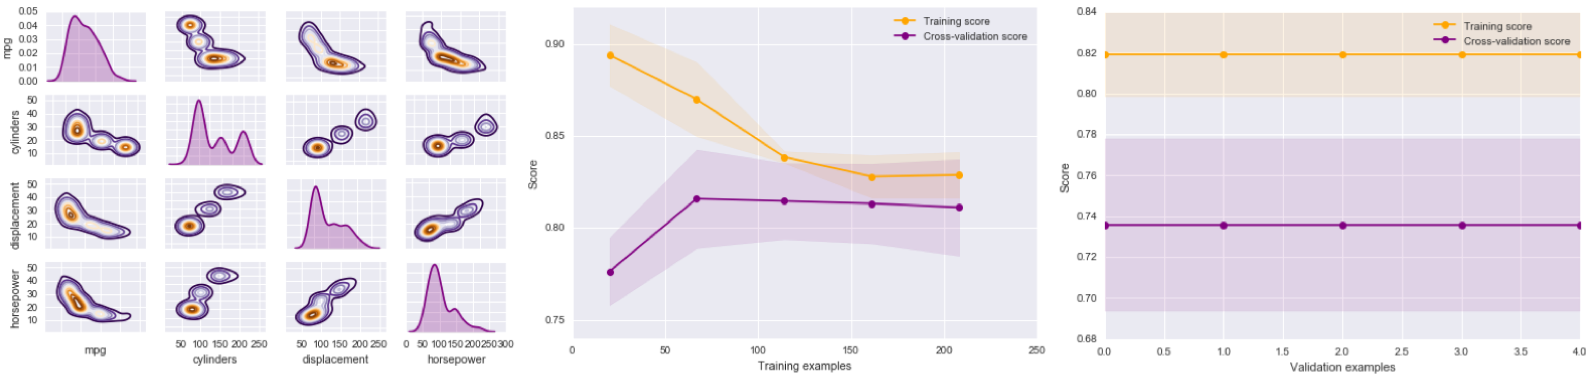
\includegraphics[width=1\textwidth]{figures/SML/auto-mpg-results.png}
\centering
\caption{The SML \(Query\) in figure \ref{fig:SML:AutoMPGQuery}  and the code in Appendix \ref{Appendix:Auto}. produce these results. The subgraph on the left is a lattice plot showing the density estimates of each feature used. The top right graph shows the model's learning curve and the graph on the lower right shows the validation curve.}
\label{fig:AutoMPG:Results}
\end{sidewaysfigure}

\clearpage


\begin{lstlisting}[language=python,  caption={Example of a SML Query Performing Classification.}, label={lst:sml-ex-1}]
READ "/path/to/data" (separator =  ";", header = None) 
AND SPLIT (train = 0.8,  test=0.2) AND CLASSIFY 
(predictors =[1,2,3,4],  label = 5, algorithm = svm) 
\end{lstlisting}


\begin{lstlisting}[language=python,  caption={Here the example \(Query\) in listing \ref{lst:sml-ex-1} is defined in BNF format.}, label={lst:SML:BNFComp}]
<Keyword> <Argument> (<OptionList>) 
AND <Keyword> (<OptionList>) AND <Keyword>
(<OptionList>) 
\end{lstlisting}

\begin{lstlisting}[language=python,  caption={Examples using the \(READ\) \(Keyword\) in SML.}, label={lst:SML:READ}]
READ "/path/to/data" 
READ "/path/to/data" (separator = ";", header = None) 
\end{lstlisting}


\begin{lstlisting}[language=python,  caption={An example utilizing the \(REPLACE\) \(Keyword\) in SML.}, label={lst:SML:REPLACE}]
READ "/path/to/data" (separator = ";", header = None) 
AND REPLACE (missing = "NaN",  strategy = "mode")
\end{lstlisting}

\begin{lstlisting}[language=python,  caption={Example using the \(SPLIT\) \(Keyword\) in SML.}, label={lst:SML:SPLIT}]
READ "/path/to/data" (separator = ";", header = None) 
AND SPLIT (train = 0.8, test = 0.2)
\end{lstlisting}

\begin{lstlisting}[language=python,  caption={Example using the \(CLASSIFY\) \(Keyword\) in SML.  Here we read in data and create training and testing datasets using the \(READ\) and \(SPLIT\) \(Keyword\)s respectively. We then use \(CLASSIFY\) \(Keyword\) with the first 4 columns as features and the 5th column to perform classification using a support vector machine.}, label={lst:SML:CLASSIFY}]
READ "/path/to/data" (separator = ";", header = None) 
AND SPLIT (train = 0.8, test = 0.2) AND CLASSIFY
(predictors = [1,2,3,4],  label=5,  algorithm=svm)
\end{lstlisting}

\begin{lstlisting}[language=python,  caption={Example using the CLUSTER Keyword in SML. Here we read in data and create training and testing datasets using the READ and SPLIT Keywords respectively. We then use CLUSTER Keyword with the first 4 columns as features and perform unsupervised clustering with the K-Means algorithm.}, label={lst:SML:CLUSTER}]
READ "/path/to/data" (separator = ";", header = None) 
AND SPLIT (train = 0.8, test = 0.2) AND  CLUSTER
(predictors = [1,2,3,4],  algorithm=kmeans)
\end{lstlisting}

\begin{lstlisting}[language=python,  caption={Example using the \(REGRESS\) \(Keyword\) in SML. Here we read in data and create training and testing datasets using the \(READ\) and \(SPLIT\) \(Keyword\)s respectively. We then use \(REGRESS\) \(Keyword\) with the first 4 columns as features and the 5th column to perform regression on using ridge regression.}, label={lst:SML:REGRESS}]
READ "/path/to/data" (separator = ";", header = None) 
AND SPLIT (train = 0.8, test = 0.2) AND  CLUSTER
(predictors = [1,2,3,4],  label=5, algorithm=ridge)
\end{lstlisting}

\begin{lstlisting}[language=python,  caption={Example using the \(LOAD\) and \(SAVE\) \(Keyword\)s in SML.}, label={lst:SML:SAVE_LOAD}]
SAVE "/path/to/save/model" 
LOAD "/path/to/save/model" 
\end{lstlisting}

\clearpage

\begin{lstlisting}[language=python,  caption={Example using the \(PLOT\) \(Keyword\) in SML.}, label={lst:SML:PLOT}]
READ "/path/to/data" (separator = ";", header = None) 
AND SPLIT (train = 0.8, test = 0.2) AND  CLUSTER
(predictors = [1,2,3,4],  algorithm=kmeans)
AND PLOT
\end{lstlisting}

\begin{lstlisting}[language=python,  caption={SML \(Query\) that performs classification on the iris dataset using support vector machines. It's important to note that detailed documentation is publicly available in \textsuperscript{\ref{lab:iris:git}} and the purpose of this figure is to highlight the level of the level of complexity relative to an SML query.}, label={lst:SML:IrisQuery}]
from sml import execute
query = 'READ "../data/iris.csv" AND \ 
SPLIT (train = 0.8, test = 0.2) AND \ 
CLASSIFY (predictors = [1,2,3,4],  label = 5, algorithm=svm) AND \
PLOT'

execute(query, verbose=True)
\end{lstlisting}

\begin{lstlisting}[language=python,  caption={SML \(Query\) that performs regression on the Auto-MPG dataset using Linear Regression.}, label={lst:SML:AutoMPGQuery}]
from sml import execute
query = 'READ "../data/auto-mpg.csv" AND \ 
REPLACE (missing = "?", strategy = "mode") AND \
SPLIT (train = 0.8, test = 0.2) AND \ 
REGRESS (predictors = [2,3,4,5,6,7,8],  label = 1, algorithm=simple) AND \
PLOT'

execute(query, verbose=True)
\end{lstlisting}



%\clearpage

%\appendix


%\clearpage
%\bibliographystyle{plainnat}
%\bibliography{thesisbib}
\bibliographystyle{plainnat}
\nobibliography{thesisbib}